\documentclass[10pt,aspectratio=169]{beamer}
% Packages
\usepackage{mathabx}
\usepackage{xcolor}
\usepackage{amsmath}
\usepackage{mathtools}
\usepackage{standalone}
\usepackage{mhchem}
\usepackage{textpos}
\usepackage{graphicx}
\usepackage{wrapfig}
\usepackage{booktabs}
\graphicspath{{images}}

% Configure template
\setbeamertemplate{navigation symbols}{}

% Theme
\usetheme[progressbar=frametitle]{metropolis}
\setbeamertemplate{caption}[numbered]
\setbeamersize{text margin left=5mm,text margin right=5mm}

% Title page details:
\title{Scientific Computing: Molecular dynamics}
\subtitle{Problemsheet 3}
\author{Jimin Kim, Christian Nix, Noah Schlenker}
\date{7. June 2024}
\institute{Technical University of Munich}

\begin{document}

% Title page frame
    \maketitle

    \addtobeamertemplate{frametitle}{}{
        \begin{textblock*}{100mm} (.945\textwidth,-.85cm)
            
\includegraphics[scale=0.14]{../template/res/tum_logo.png}
        \end{textblock*}}

% Outline frame
    \begin{frame}{Outline}
        \tableofcontents
    \end{frame}

% Slides
    
\section{XML Adaptation}
\label{sec:xml}

\begin{frame}
    \frametitle{XML Format Adaptation}

    \begin{itemize}
        \item We defined XML structure and constraints using XSD .
        \item Key elements: Standard parameters, linked-cell grid specifications, boundary conditions
    \end{itemize}

    \textbf{XSD CMake flags}:
    \begin{itemize}
        \item cxx-tree
        \item --hxx-suffix=.h, --cxx-suffix=.cpp
        \item --std=c++11
        \item --generate-doxygen, --generate-serialization
    \end{itemize}
\end{frame}

    
\section{Linked-cell Algorithm}
\label{sec:lc}

\begin{frame}
    \frametitle{Cell and Cell grid}

    \begin{itemize}
        \item Realized Linked-cell through implementation of cell and cell grid
        \item Embedded into project via new simulation class and force calculation
    \end{itemize}
    \begin{figure}
        \label{fig:umlsim}
        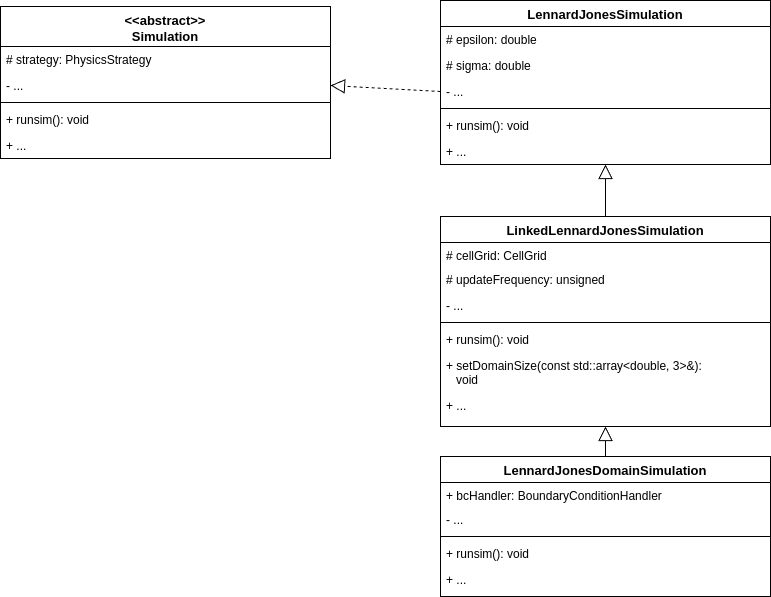
\includegraphics[width=0.5\textwidth]{res/UMLSimulation3.drawio}
    \end{figure}
\end{frame}

    
\section{Cell}
\label{sec:cell}

\begin{frame}
    \frametitle{New class Cell}
    \textbf{Contains:}
    \begin{itemize}
        \item List of particle references
        \item Type: Inner, Boundary, Halo
        \item Iterator for unique pairs over the list
    \end{itemize}
    
    \textbf{For Iteration in the grid:} \texttt{neighborCounter} and Information over position of neighbors
\end{frame}

    
\section{Cell grid}
\label{sec:grid}

\begin{frame}
    \frametitle{Linking cells in a grid}
    3D vector matrix of \texttt{std::unique\_ptr} to cells
    \begin{itemize}
        \item Initialization through specifications in XML file
        \item Assigns particle references of cells to particles in the particle container
        \item \textbf{Key function:} Get indices of relevant neighbor cells
    \end{itemize}
\end{frame}

\begin{frame}
    \frametitle{getNeighborCells}
    Algorithm to utilize newton's third law needed on cell iteration level!\newline
    $\longrightarrow$ \texttt{std::list<CellIndex> getNeighborCells(const Cellindex)}
    \begin{itemize}
        \item Distinguish between neighbor pairs, that already have been included in calculations
        \item Given an index to a cell, iteration over each neighboring cell
        \item If \textbf{neighbor cell's counter = 0}: Increment parameter cell's counter and add neighbor cell's index to return list
        \item If \textbf{neighbor cell's counter $>$ 0}: Decrease neighbor cell's counter and ignore the cell.
    \end{itemize}
\end{frame}

\begin{frame}
    \frametitle{Project Expansion}
    \begin{figure}
        \label{fig:umlcellgrid}
        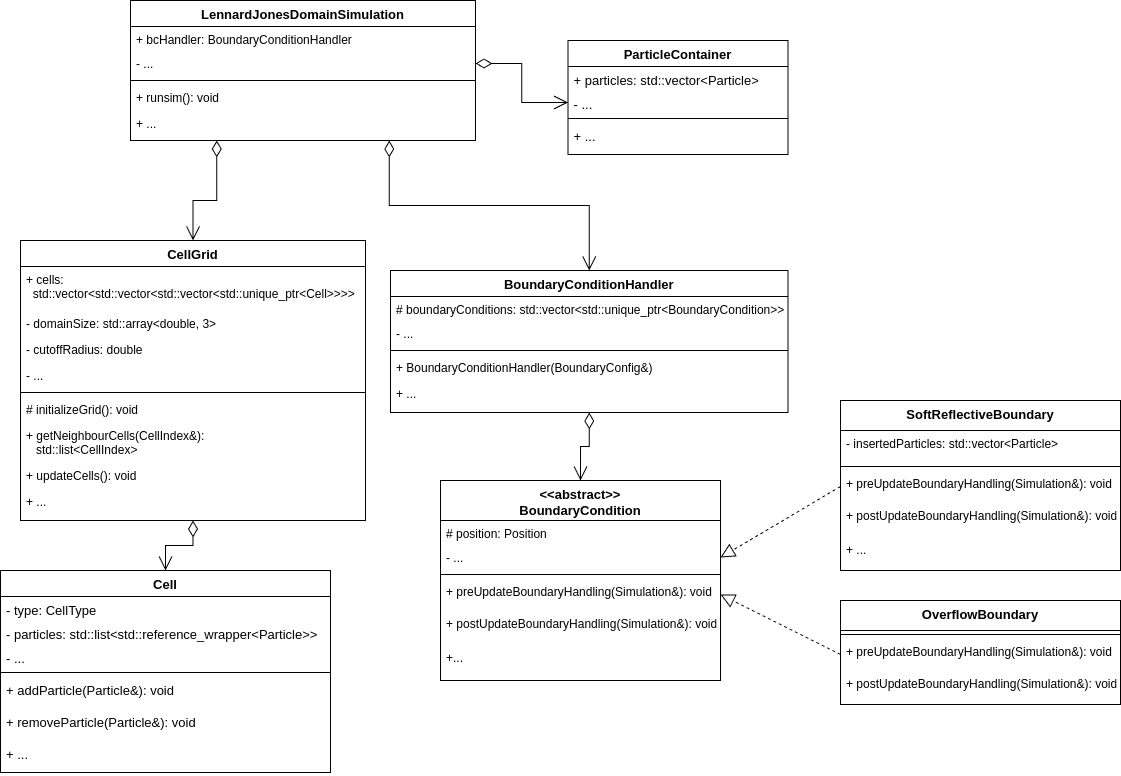
\includegraphics[width=0.7\textwidth]{res/UML3.drawio}
    \end{figure}
\end{frame}
    
\section{Performance test}
\label{sec:perf}

\begin{frame}
    \frametitle{Google Benchmark}
    \begin{table}
        \centering
    \begin{tabular}{|c|c|c|c|}
        \toprule
        Benchmark/\#Particles & Time & CPU & Iterations \\
        \toprule
        BM\_LJSimulation/1000 & 1.4485e+10 ns & 1.4477e+10 ns & 1 \\
        \midrule
        BM\_LJSimulation/2000 & 5.7983e+10 ns & 5.7959e+10 ns & 1 \\
        \midrule
        BM\_LJSimulation/4000 & 2.3180e+11 ns & 2.3171e+11 ns & 1 \\
        \midrule
        BM\_LJSimulation/8000 & 9.2722e+11 ns & 9.2686e+11 ns & 1 \\
        \midrule
        BM\_LJSimulation\_BigO & 14487.81 $N^2$ & 14482.20 $N^2$ & - \\
        \midrule
        BM\_LinkedLJSimulation/1000 & 28515871 ns & 28493193 ns & 25 \\
        \midrule
        BM\_LinkedLJSimulation/2000 & 54951418 ns & 54934137 ns & 13 \\
        \midrule
        BM\_LinkedLJSimulation/4000 & 114455900 ns & 114424760 ns & 6 \\
        \midrule
        BM\_LinkedLJSimulation/8000 & 236827726 ns & 236733811 ns & 3 \\
        \midrule
        BM\_LinkedLJSimulation\_BigO & 29304.28 $N$ & 29293.31 $N$ & - \\
        \bottomrule
    \end{tabular}
    \end{table}
\end{frame}

\begin{frame}
    \frametitle{Graphs}
    \textbf{Results show improvement from squared to linear runtime!}
    \begin{figure}
        \label{fig:timelc}
        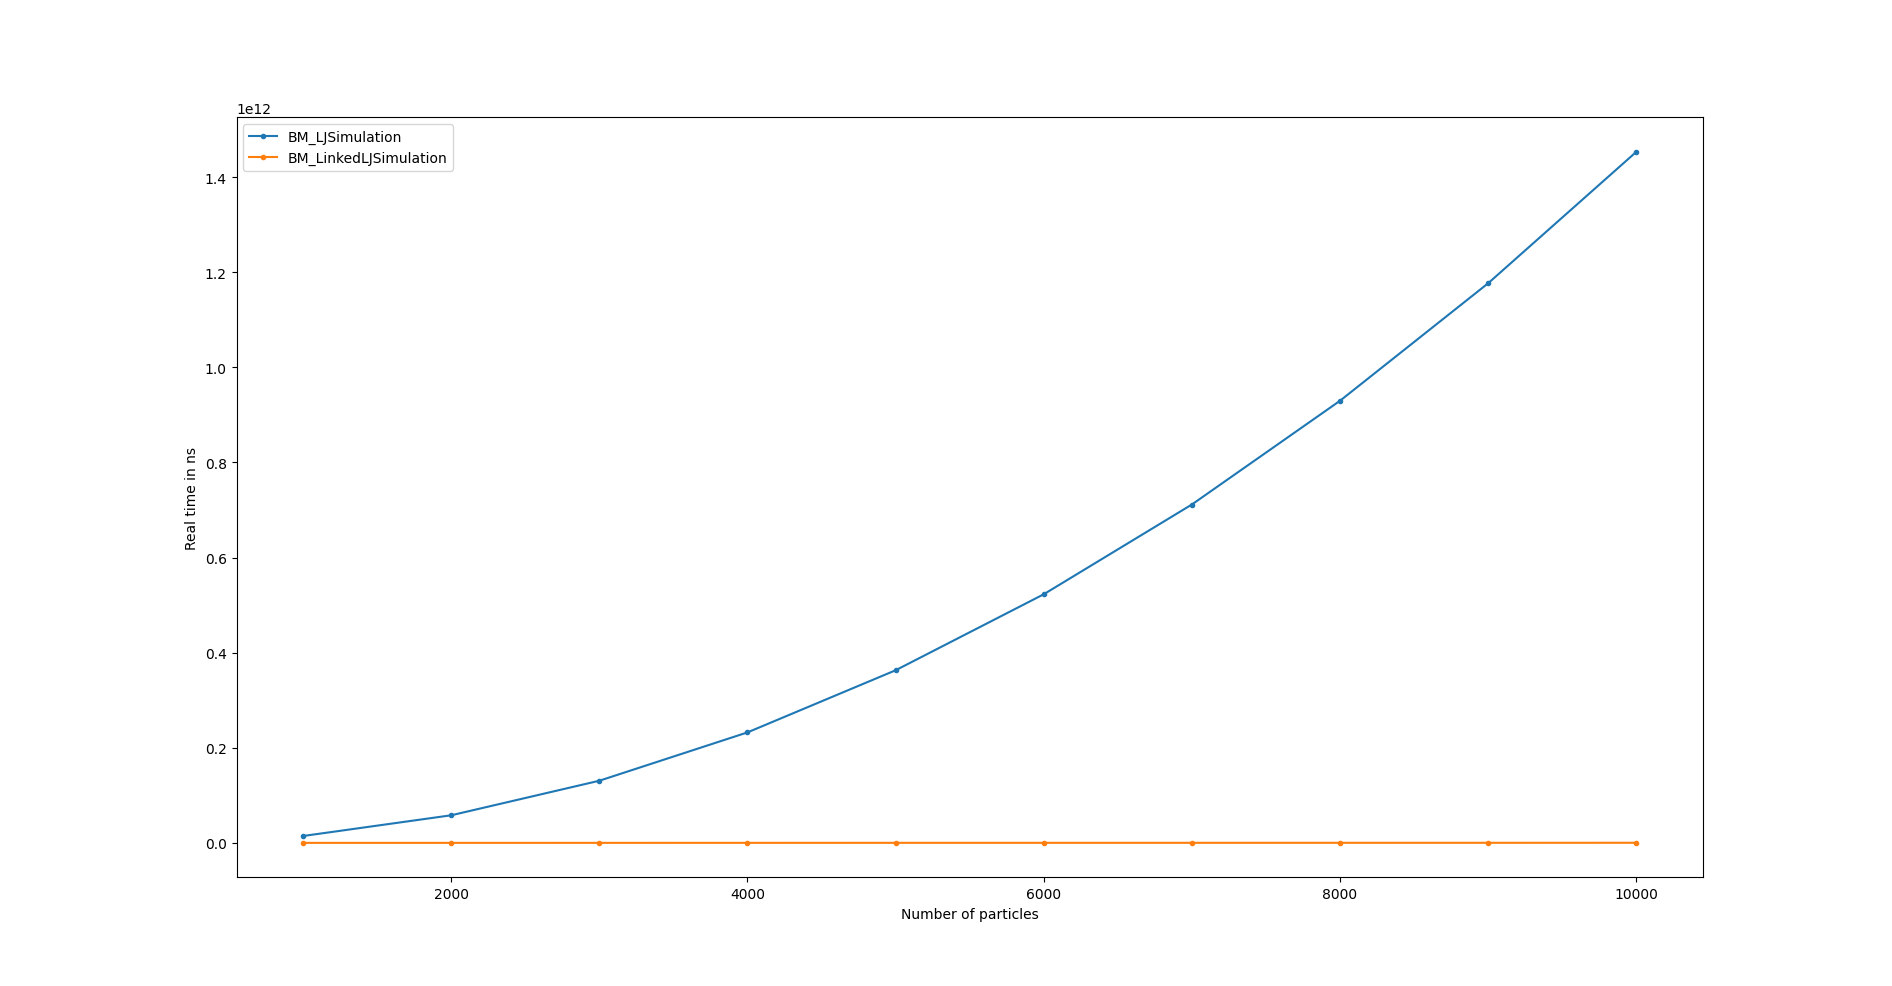
\includegraphics[width=0.9\textwidth]{res/lj_big_plot_linear}
    \end{figure}
\end{frame}

\begin{frame}
    \frametitle{Graphs}
    \begin{figure}
        \label{fig:timelclog}
        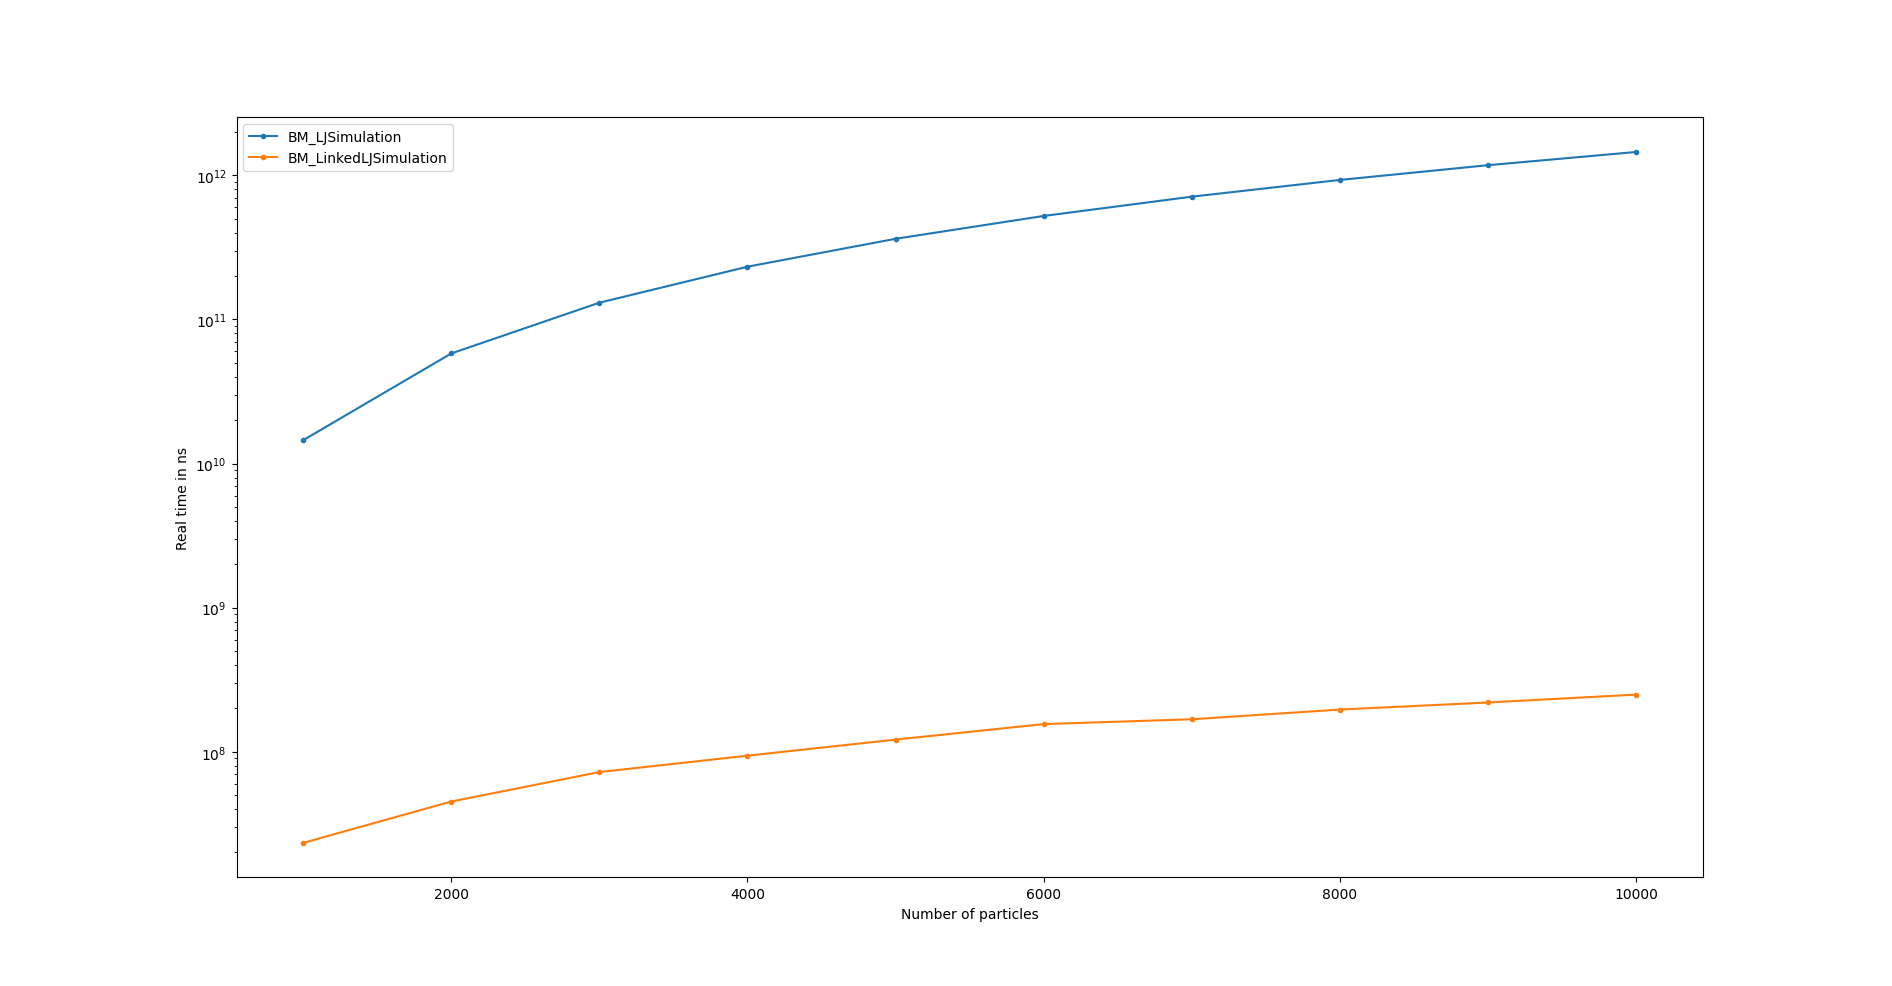
\includegraphics[width=0.9\textwidth]{res/lj_big_plot_log}
    \end{figure}
\end{frame}

    
\section{Boundary Conditions}
\label{sec:boundary}

\begin{frame}
    \frametitle{Boundary Conditions}
    \begin{itemize}
        \item Integration on simulation level
        \item Initialization from XML file via Boundary condition handler and configuration file
        \item Pre- and post-update functions: Determine particles in question and apply boundary condition
        \item \textbf{Two implementations:}
        \begin{itemize}
            \item OverflowBoundary: Particles leaving boundary get stuck and permanently ignored
            \item SoftReflectiveBoundary: Particles reflect against ghost particles
        \end{itemize}
    \end{itemize}
\end{frame}

    
\section{Sphere generation}
\label{sec:sphere}

\begin{frame}
    \frametitle{Sphere Particle Cluster}
    Extension of our generators \newline
    \textbf{Idea:}
    \begin{itemize}
        \item 2D Discs: Concentric rings of particles
        \item 3D Sphere: Stack of discs
        \item Trigonometric functions for even spacing of particles
    \end{itemize}
\end{frame}

\begin{frame}
    \frametitle{Trigonometric functions}
    \textbf{Angular step calculation:}
    \begin{itemize}
        \item Angular step $\theta$ between particles for spacing at least at a given distance along the circumference.
        \item Given a ring with radius \textit{r} and particle spacing \textit{s}, the angular step $\theta$ is determined by:
        \item $\theta = 2 \arcsin\left(\frac{s}{2 \times r}\right)$
    \end{itemize}
    \textbf{Number of particles calculation:}
    \begin{itemize}
        \item The number of particles \textit{N} given by dividing the full circle ($2\pi\ radians$) by the angular step $\theta$:
        \item $N = \left\lfloor \frac{2\pi}{\theta} \right\rfloor$
    \end{itemize}
    \textbf{Positioning of particles:}
    \begin{itemize}
        \item Calculation using polar coordinates, for a particle at index \textit{i}:
        \item $x_i = \text{origin}_x + r \cos(i \theta)\newline y_i = \text{origin}_y + r \sin(i \theta)\newline z_i = \text{origin}_z + \text{z\_offset}$
    \end{itemize}
\end{frame}

\begin{frame}
    \frametitle{Final Sphere}
    \begin{figure}
        \label{fig:sphere}
        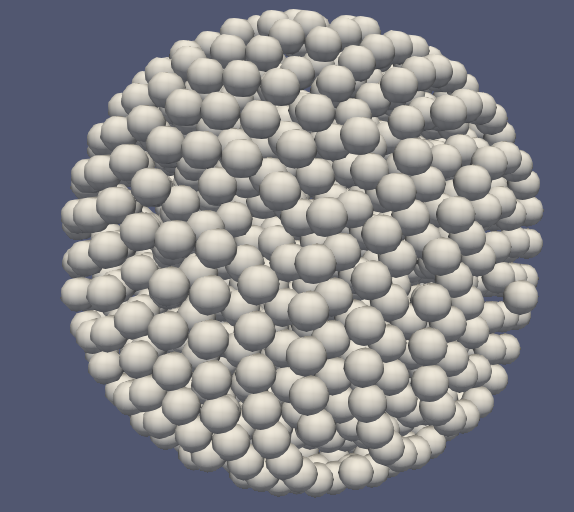
\includegraphics[width=0.5\textwidth]{res/sphere}
    \end{figure}
\end{frame}

\end{document}